\documentclass[12pt,a4paper,]{article}
\usepackage[]{kpfonts}
\usepackage{amssymb,amsmath}
\usepackage{ifxetex,ifluatex}
\usepackage{fixltx2e} % provides \textsubscript
\ifnum 0\ifxetex 1\fi\ifluatex 1\fi=0 % if pdftex
  \usepackage[T1]{fontenc}
  \usepackage[utf8]{inputenc}
\else % if luatex or xelatex
  \ifxetex
    \usepackage{mathspec}
  \else
    \usepackage{fontspec}
  \fi
  \defaultfontfeatures{Ligatures=TeX,Scale=MatchLowercase}
\fi
% use upquote if available, for straight quotes in verbatim environments
\IfFileExists{upquote.sty}{\usepackage{upquote}}{}
% use microtype if available
\IfFileExists{microtype.sty}{%
\usepackage{microtype}
\UseMicrotypeSet[protrusion]{basicmath} % disable protrusion for tt fonts
}{}
\usepackage[margin=1in]{geometry}
\usepackage{hyperref}
\hypersetup{unicode=true,
            pdftitle={Calculating the Housing Wealth Effect of Israeli regional cohorts},
            pdfauthor={Brandon Payne},
            pdfborder={0 0 0},
            breaklinks=true}
\urlstyle{same}  % don't use monospace font for urls
\usepackage[style=authoryear-comp]{biblatex}

\addbibresource{currentEcon.bib}
\usepackage{longtable,booktabs}
\usepackage{graphicx,grffile}
\makeatletter
\def\maxwidth{\ifdim\Gin@nat@width>\linewidth\linewidth\else\Gin@nat@width\fi}
\def\maxheight{\ifdim\Gin@nat@height>\textheight\textheight\else\Gin@nat@height\fi}
\makeatother
% Scale images if necessary, so that they will not overflow the page
% margins by default, and it is still possible to overwrite the defaults
% using explicit options in \includegraphics[width, height, ...]{}
\setkeys{Gin}{width=\maxwidth,height=\maxheight,keepaspectratio}
\IfFileExists{parskip.sty}{%
\usepackage{parskip}
}{% else
\setlength{\parindent}{0pt}
\setlength{\parskip}{6pt plus 2pt minus 1pt}
}
\setlength{\emergencystretch}{3em}  % prevent overfull lines
\providecommand{\tightlist}{%
  \setlength{\itemsep}{0pt}\setlength{\parskip}{0pt}}
\setcounter{secnumdepth}{5}

%%% Use protect on footnotes to avoid problems with footnotes in titles
\let\rmarkdownfootnote\footnote%
\def\footnote{\protect\rmarkdownfootnote}

%%% Change title format to be more compact
\usepackage{titling}

% Create subtitle command for use in maketitle
\newcommand{\subtitle}[1]{
  \posttitle{
    \begin{center}\large#1\end{center}
    }
}

\setlength{\droptitle}{-2em}
  \title{Calculating the Housing Wealth Effect of Israeli regional cohorts}
  \pretitle{\vspace{\droptitle}\centering\huge}
  \posttitle{\par}
  \author{Brandon Payne}
  \preauthor{\centering\large\emph}
  \postauthor{\par}
  \date{}
  \predate{}\postdate{}

\usepackage{benyominwp}

% META DATA

\wp{Housing Wealth Effect Proposal}

%\jel{C10,C14,C22}

\addresses{
\textbf{Brandon Payne}\\
                Woodman-Scheller Israel Studies International Program\\
                Ben-Gurion University of the Negev\\
                Email: payneb@post.bgu.ac.il\\[1cm]
}

\lfoot{\sf Payne: \Date~\Month~\Year}

\begin{document}
\maketitle

\begin{abstract}
Uses pseudo-panel construction to calculate the housing wealth effect for regional cohorts of Isreali households. Combines data from the Central Bureau of Statistics Household Expenditure Survey and the Consumer Price Index.
\end{abstract}

\begin{keywords}
 consumption, economics, housing, housing market, liquidity constraints, wealth effect 
\end{keywords}

\newpage

\section{Introduction}\label{introduction}

\subsection{The housing market}\label{the-housing-market}

The study of housing provides a fascinating topic for the researcher of
Israeli society. Several factors have drawn attention to the housing
market and made it a topic of much discussion. The price of housing was
one of the main issues that drove more than 400,000 demonstrators to the
streets in the summer of 2011. Large portions of the Israeli population
own a home, or rent one, or live in a multi-family household. Their
first-hand experience of the market may be relayed to the researcher as
anecdotal evidence of the state of the housing market, as well as causes
and solutions for the perceived short-comings of the market.

In a simple economic model of a housing market, home prices are set by
the market forces of supply and demand. Various factors influence the
supply and demand of housing in the market. Consider an interest-rate
reduction, this shifts the demand curve to the right, as cheaper credit
entices more buyers to enter the market. It also reduces
credit-constraints on builders and leads to increased supply, albeit
after some lag. In Israel, the average home price has risen by an
astonishing 80\% between the 2008 global financial crisis and 2016. In
the minds of many lay observers this rapid increate indicates a lack of
supply. Main bottlenecks limiting supply are cited as the sale of
government land or the lengthy permitting process for new construction.

Gruber \autocite{gruberSep2016}, however, offers copious evidence and
cogent reasoning to support his claim that the chief factor in the rise
was actually excessive demand. As global capital markets suffered large
declines, investors moved to other asset classes, including the real
estate market. The additional factor of low interest rates lead to a
dramatic increase in purchase of additional houses by those who were
already owner-occupiers. This shifted the demand curve to the right,
increasing the average cost of an apartment and driving out less
affluent first-time homebuyers. These would-be first-time homebuyers
then entered or remained in the rental market, driving up average rents.
The higher market rental prices and lowered vacancy rate established a
feedback loop which further encouraged in the purchase of investment
houses as rental property.

\subsection{Consumption by Households}\label{consumption-by-households}

The expenditure method for calculating National Income (Y), states that
Y=GDP=C+I+G+NX. The gross domestic product is equal to Consumption
Expenditure (C) plus Investment Expenditure (I) plus Government
Expenditure (G) plus Net Exports (NX). Firms and households each engage
in both consumption and investment. When a firm buys a copy machine
which lasts several years, that is an investment. The purchase of
owner-occupied housing is the largest investment made by most
households. The paper placed in the copy machine and the food on the
table are each classified as consumption. Consumption by households
makes up a large and important part of GDP, as seen in figure 1.
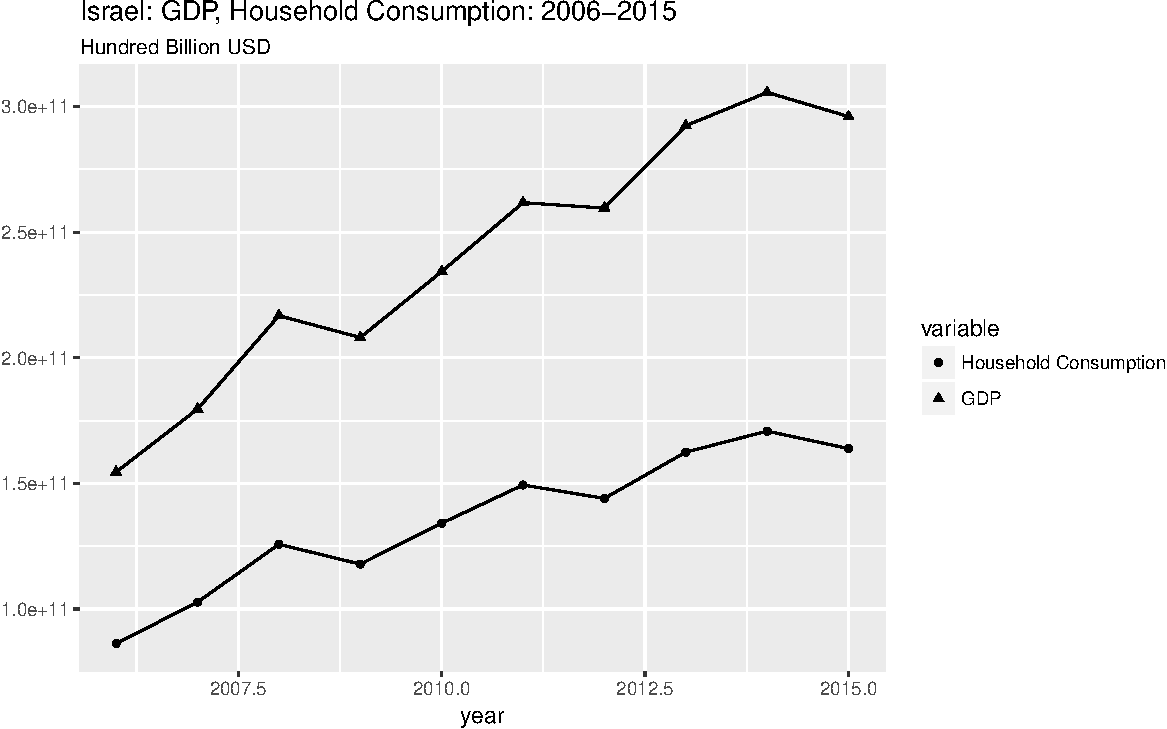
\includegraphics{currentWorkingDraft_files/figure-latex/unnamed-chunk-1-1.pdf}

As can be seen from the graph, in 2015 Household Consumption was 55.3\%
of GDP. If the housing wealth effect is large is, its effect on this
large portion of the economy will have real, import, reaching effects in
people's lives. It is a measure tracked closely by businesses,
economists and the government.

Household income is either saved or consumed, with the marginal
propensity to consume (MPC) and the marginal propensity to save (MPS)
summing to 1. Generally, household consumption can be understood as
household income times the MPC. The MPC can be affected by the interest
rate, rising interest rates incentivize additional savings, raising the
MPS and lowering the MPC. Falling interest rates decrease the attraction
of savings. With a constant MPC a household can increase consumption due
to increased income from a salary increase, hourly wage increase or
increase in the number of hours worked. Household consumption would fall
due a decrease in salary, wages or working hours. A further factor in
consumption is expected future income. This posits that the rational
consumer increases their consumption now if they know that they will get
a raise or some overtime next week. They will also reduce consumption
and increase savings now when they expect future unemployment or wage
reductions. Another factor affecting consumption is the wealth effect.
When the wealth of a household increases (the price of shares held in an
investment portfolio, the price of a Picasso on the wall or in a vault,
the price of the family home or rental property), household consumption
increases, in effect spending now some of the expected future gains on
the sale of the shares, painting or real estate. Conversely, a decline
in household wealth should produce a decline in household consumption.

\section{Literature Review}\label{literature-review}

\subsection{the housing wealth effect}\label{the-housing-wealth-effect}

Many households around the world store a majority of their wealth in
housing. This, combined with the volatility of swings in house prices,
has caused academics and policy makers to further investigate the
housing wealth effect and its implications for GDP.\autocite{Gan2010}
Renters and owners should be effected differently by a change in housing
prices. An increase in housing prices should increase consumption by
owners and decrease consumption by renters. Changes in house prices
affect renters through the mechanism of the savings motive. One of the
factors influencing the renter's mix of savings and consumption is their
desire to purchase a home in the future. Renters respond to an increase
in the price of housing by adjusting their expectation of the future
price of the home they wish to purchase. They then reduce their
consumption and increase their savings rate. Research using Japanese
data showed that renters fell into two categories when faced with
increased housing prices. Some gave up saving for a home and instead
increased consumption of luxury goods in what was termed the
``consumption of despair.'' The other group decreased consumption, and
increased their savings rate, still dreaming of home ownership. These
effects on renters were subsequently found in data from Canada and San
Francisco.\autocite{Sheiner_1995}

The data used in the proposed study should allow me to measure the
extent to which Israeli renters engaged in consumption of despair over
the last fourteen years. The life cycle savings hypothesis suggests that
consumption of anticipated increases in wealth will be distributed by
consumers over time, and that there would be a single MPC for both
housing wealth and stock market wealth. When empirically tested, data
showed that 85\% of respondents did not increase consumption in response
to a change in their shares portfolio. Several reasons were suggested
why changes in the value of wealth held in different forms would illicit
different consumption effects from households. Prices changes in some
assets may be viewed as transitory. Others may be harder to measure than
the daily feedback of the stock quote. Tax laws may discourage the sale
of certain assets and wealth may be held in separate ``mental
accounts,'' one of which may be a rainy-day fund against life's
uncertainties.

\subsection{Mechir Lamistaken - The Israeli first-time homebuyers
program}\label{mechir-lamistaken---the-israeli-first-time-homebuyers-program}

Finance Minister Moshe Kahlon has a plan to deal with the excess demand
in the housing market caused by real estate speculators who would own
one apartment and still buy one or more others as rental property. The
Mechir Lamistaken program sells land to developers at a below market
rate if the housing is reserved for first-time buyers. However, there is
evidence for widespread use by investors of strawbuyers to evade the
restriction. Thus, young families are still squeezed out of the market
and the government forgoes revenue from land sales while benefiting
investors. An important factor that reduces the supply of housing by
increasing permitting times for new construction is the lack of
municipally determined property tax rates. New residential units add an
additional burden on city infrastructure and do not pay for themselves
in terms of the taxes they generate. Wealthier districts make up the
short fall through taxes on commercial property. Poorer localities throw
up additional barriers to delay the construction of apartments until
they are promised balance grants by the Ministry of Interior.

\section{Methodology}\label{methodology}

This research is being conducted in the interdisciplinary field of
Israel Studies. It lies at the intersection of sociology and economics.
It partially adheres to the practices of reproducible research,
i.e.~methods are fully reported and the process by which raw data is
anaylzed is viewable. Unfortunately, while the housing price data is
freely distributable, the household level consumption data is not. This
is fully reproducible after obtaining the listed datasets, which are
available from the Central Bureau of Statistics and the Israel Social
Sciences Data Center. Pseudo-panel construction is the methodology by
which I propose to combine the available data on household consumption
and house prices.

\subsection{data sets}\label{data-sets}

This study combines household level consumption data with housing price
data to estimate test the hypothesis that different age cohorts have
different wealth effects. It has been postulated that older households
will have a higher wealth effect, or larger proportional change in
spending in response to a change in wealth than a younger household. The
available consumption data from the Household Expenditure Survey
provides us with a means to test this hypothesis. Table One shows a
listing of the files used in the study. Column 2 - Consumption, names
the files from the ``Housing Expenditure Survey.'' Column 3 shows the
locations of the housing price data. These are data are released as part
of the calculation of the Consumer Prices Index as Table 6.2 - ``Average
Prices of Owner Occupied Dwellings (NIS Thousand), by Residential Area
and Size Groups (Rooms in Dwelling).'' The data for the fourteen years
in question, 2002-2015 is split among six files that are at different
locations, but all named the same thing. These files each contain 8
quarters of data. They are renamed upon download and saved with the
filenames in column four. The nine Residental Areas are Jerusalem, Tel
Aviv, Haifa, Gush Dan, Center, South, Sharon, North and Qrayot Haifa.
Apartments are grouped by number of rooms, 1.5-2, 2.5-3, 3.5-4 and
4.5-5. Also included is an average home price for the Residential Area.
This is not an average of the four size groups. These data from the
various years are then combined to produce a time-series of home prices
from 2002 to 2015 for the nine location/size pairs.

\begin{tabular}{l|l|l|l}
\hline
years & Consumption & www.cbs.gov.il/www/ + & houseP\_savedAs\\
\hline
2002 & requested & MISSING & NA\\
\hline
2003 & requested & MISSING & NA\\
\hline
2004 & requested & MISSING & NA\\
\hline
2005 & f467 & archive/200803/price\_new/a6\_2\_e.xls & NA\\
\hline
2006 & f468 & archive/200803/price\_new/a6\_2\_e.xls & houseP06\_07.xls\\
\hline
2007 & f469 & archive/201003/price\_new/a6\_2\_e.xls & houseP06\_07.xls\\
\hline
2008 & requested & archive/201003/price\_new/a6\_2\_e.xls & houseP08\_09.xls\\
\hline
2009 & f472 & archive/201203/price\_new/a6\_2\_e.xls & houseP08\_09.xls\\
\hline
2010 & f471 & archive/201203/price\_new/a6\_2\_e.xls & houseP10\_11.xls\\
\hline
2011 & f459 & archive/201403/price\_new/a6\_2\_e.xls & houseP10\_11.xls\\
\hline
2012 & f458 & archive/201403/price\_new/a6\_2\_e.xls & houseP12\_13.xls\\
\hline
2013 & f457 & archive/201503/price\_new/a6\_2\_e.xls & houseP12\_13.xls\\
\hline
2014 & f456 & /price\_new/a6\_2\_e.xls & houseP14\_16.xls\\
\hline
2015 & requested & /price\_new/a6\_2\_e.xls & houseP14\_16.xls\\
\hline
\end{tabular}

\clearpage
<!-- <--- \nocite{*} --> --\textgreater{}

\printbibliography


\end{document}
